\subsection{Problem~1}%
\label{problem:1}

Check the first- and second-order optimality conditions at the point
$\matr{x}^* = \begin{bmatrix} 1 \\ 1 \end{bmatrix}$
of the Rosenbrock function:
\begin{equation*}
  f(\matr{x}) = 100(x_2 - x_1^2)^2 + (1-x_1)^2.
\end{equation*}
Draw a contour plot of this function.

\subsubsection*{Mathematics}

In unconstrained optimization we seek $\matr{x}^*$ minimising $f : \mathbb{R}^N \to \mathbb{R}$
with no restrictions on $\matr{x}$.
A point $\matr{x}^*$ is a \textit{local minimizer} if there exists a neighbourhood
$\mathcal{N}$ of $\matr{x}^*$ such that $f(\matr{x}^*) \leq f(\matr{x})$ for all
$\matr{x} \in \mathcal{N}$.

\textbf{Theorem (First-order necessary condition).}
If $\matr{x}^*$ is a local minimizer and $f$ is continuously differentiable in an open
neighbourhood of $\matr{x}^*$, then $\nabla f(\matr{x}^*) = \matr{0}$ \citep{NoceWrig99}.

\textbf{Theorem (Second-order necessary condition).}
If additionally $\nabla^2 f$ is continuous near $\matr{x}^*$, then the Hessian
$\nabla^2 f(\matr{x}^*)$ must be \textit{positive semi-definite}.

\textbf{Theorem (Second-order sufficient condition).}
If $\nabla f(\matr{x}^*) = \matr{0}$ and $\nabla^2 f(\matr{x}^*)$ is
\textit{positive definite}, then $\matr{x}^*$ is a \textit{strict local minimizer}.
Positive definiteness is verified via Sylvester's criterion: all leading principal
minors $M_k > 0$.

\subsubsection*{Solution}

The partial derivatives of the Rosenbrock function are:
\begin{align*}
  \frac{\partial f}{\partial x_1} &= -400 x_1(x_2 - x_1^2) - 2(1-x_1), \\
  \frac{\partial f}{\partial x_2} &= 200(x_2 - x_1^2).
\end{align*}
At $\matr{x}^* = [1,1]^T$: $x_2 - x_1^2 = 0$ and $1 - x_1 = 0$, hence
\begin{equation*}
  \nabla f(\matr{x}^*) = \begin{bmatrix} 0 \\ 0 \end{bmatrix}.
\end{equation*}
The first-order condition is satisfied --- $\matr{x}^*$ is a stationary point.

The Hessian of $f$ is:
\begin{equation*}
  \nabla^2 f(\matr{x}) =
  \begin{bmatrix}
    1200 x_1^2 - 400 x_2 + 2 & -400 x_1 \\
    -400 x_1 & 200
  \end{bmatrix}.
\end{equation*}
Evaluating at $\matr{x}^* = [1,1]^T$:
\begin{equation*}
  H = \begin{bmatrix} 802 & -400 \\ -400 & 200 \end{bmatrix}, \qquad
  M_1 = 802 > 0, \qquad
  M_2 = \det(H) = 802 \cdot 200 - 400^2 = 400 > 0.
\end{equation*}
Both leading principal minors are positive, so $H$ is positive definite.
By the second-order sufficient condition, $\matr{x}^* = [1,1]^T$ is a
\textbf{strict local (and global) minimizer} of the Rosenbrock function.

\lstinputlisting[style=Matlab-editor]{problems/Problem_1.m}

\begin{figure}[H]
  \centering
  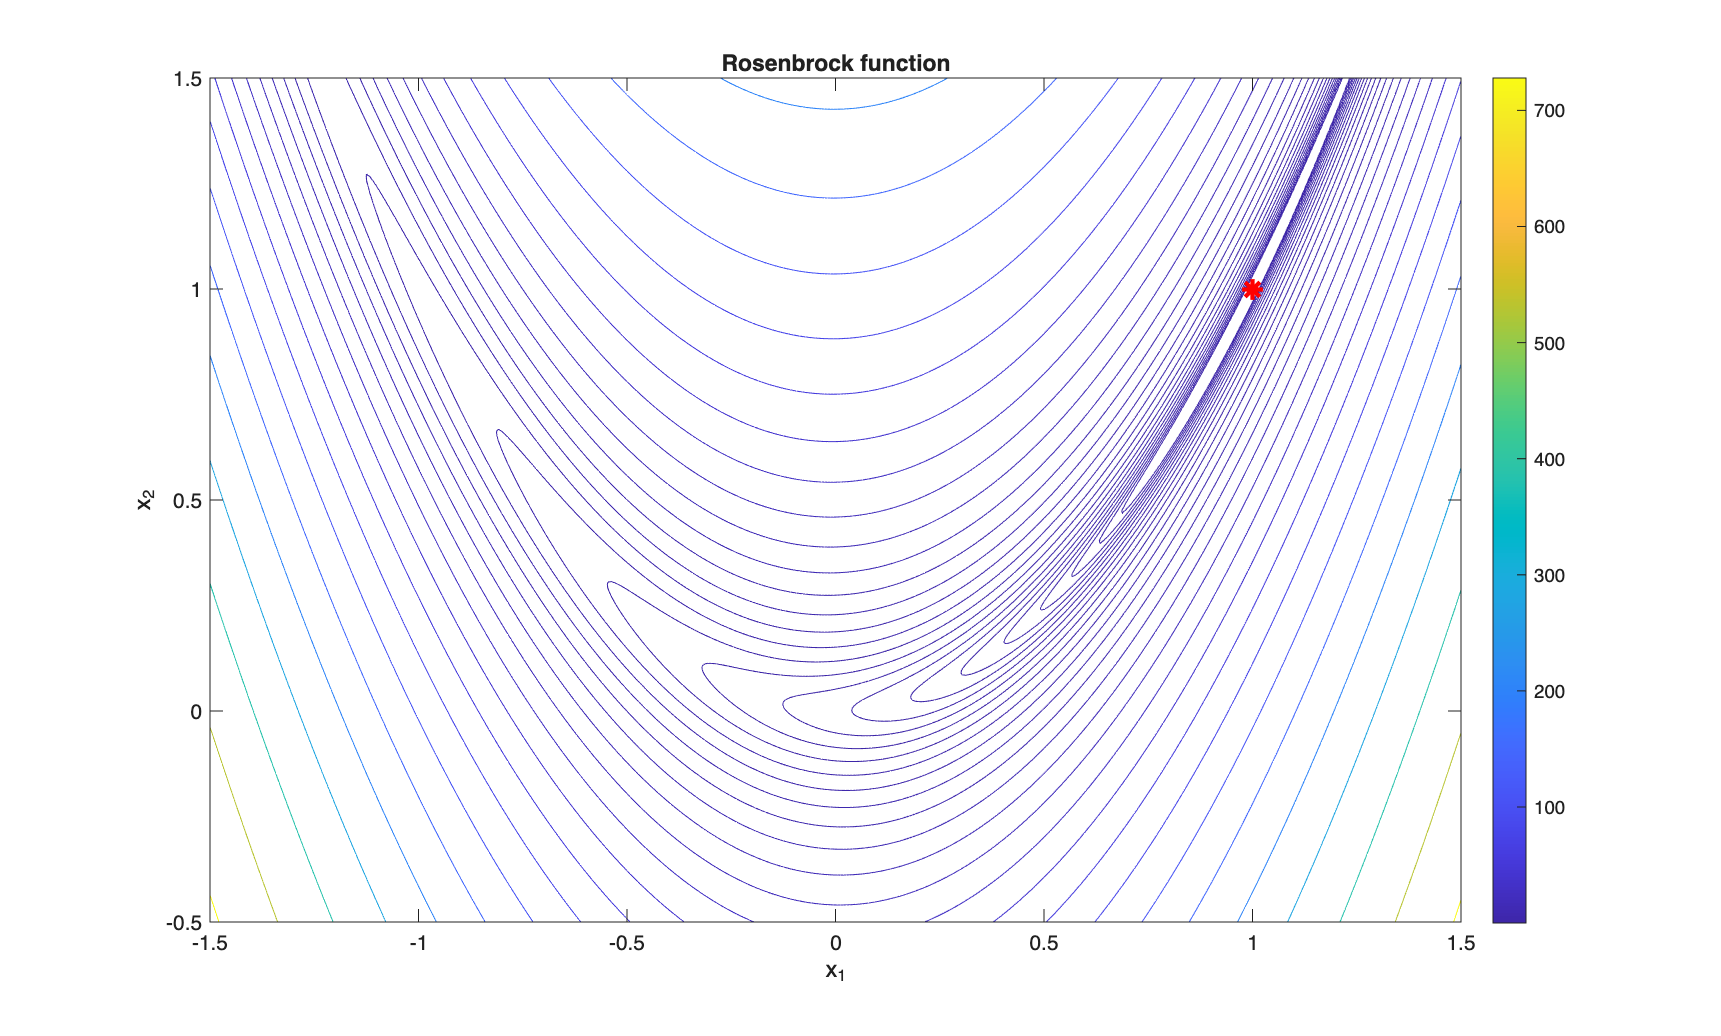
\includegraphics[width=0.75\textwidth]{images/Contour_Problem1.png}
  \caption{Contour plot of the Rosenbrock function.
    The global minimizer $\matr{x}^* = [1,1]^T$ is marked with a red star.}
\end{figure}
